\chapter{Background}
\renewcommand{\baselinestretch}{\mystretch}
\label{chap:BG}
%\setlength{\parindent}{0pt}

\section{Vixen overview}

\PARstart{T}{he} Vixen application was based on Microsoft Windows .NET runtime \cite{dotnet}, developed using Microsoft Visual Studio \cite{msvs}. It is capable of loading modules as dynamic-link libraries (DLL) during runtime. Most of its components such as controllers, lighting effects and editor were implemented as separate modules. \fref{fig:vixen-main} shows the main application interface.

\begin{figure}[!t]
  \centering
  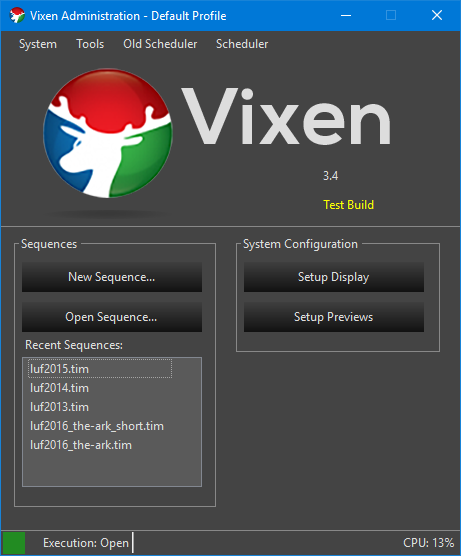
\includegraphics[width=0.6\textwidth]{Figs//vixen_main.png}
  \caption{\footnotesize Main entry GUI of Vixen application}
  \label{fig:vixen-main}
\end{figure}

The execution engine consists of 4 stages for flexible and intuitive lighting sequence editing, as shown in \fref{fig:stages}.

\begin{figure}[!t]
  \centering
  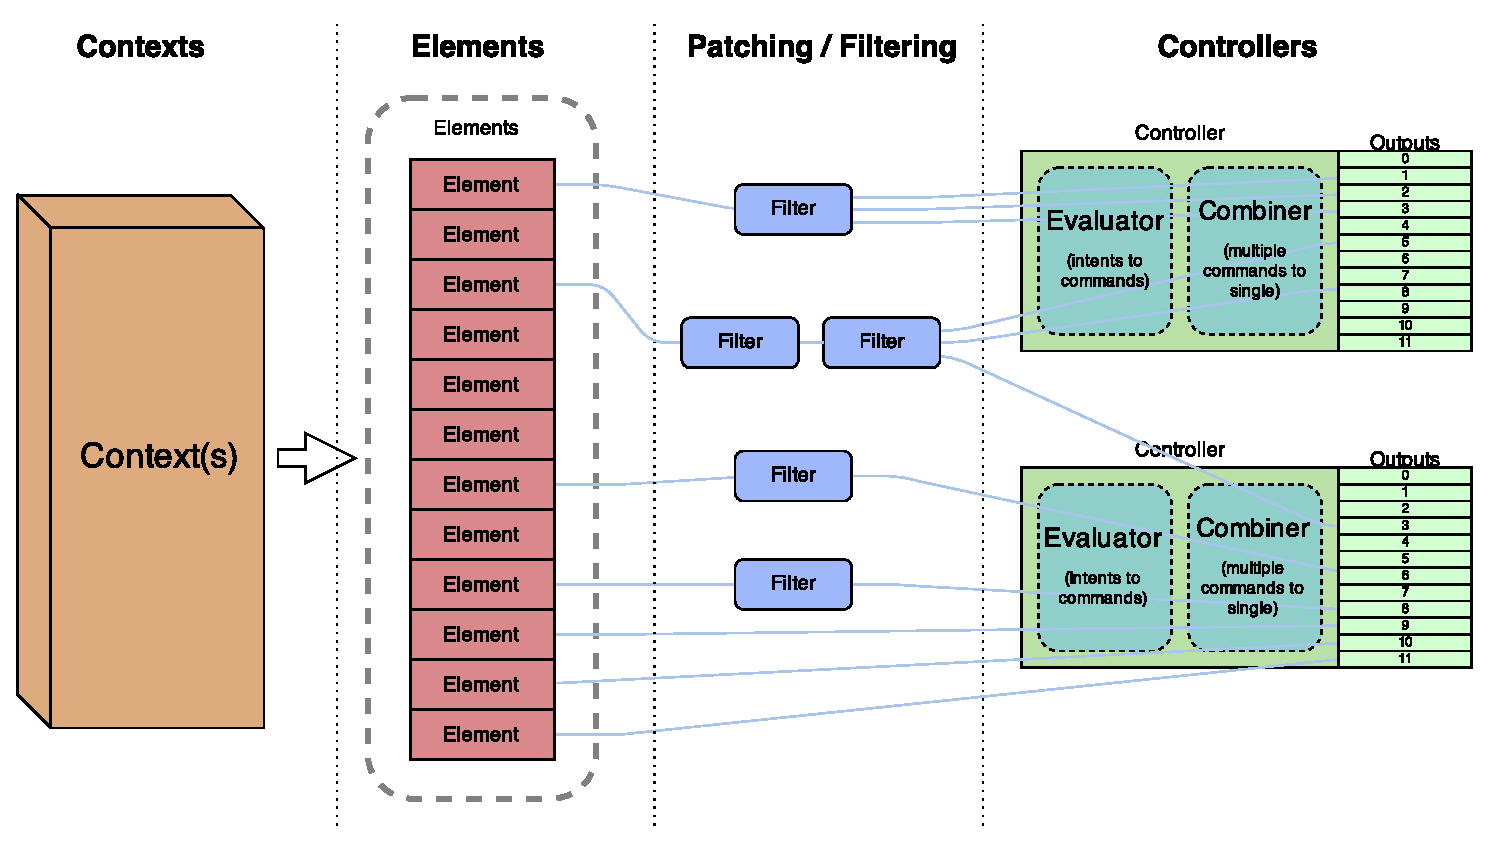
\includegraphics[width=0.85\textwidth]{Figs//V3-Engine-1.eps}
  \caption{\footnotesize Vixen execution engine stages (adopted from \cite{vixen})}
  \label{fig:stages}
\end{figure}

Contexts are at the very top level of data structures used by Vixen. Vixen stores lighting effects by sequence files, each sequence represents a context to be executed. By using a built-in show scheduler, Vixen can load, pre-render and cache multiple sequence contexts at the same time, then scheduled to be repeatedly played afterwards.

Each sequence context contains lots of elements. Elements represent abstract items described by the user. For example, lights on trees, lights on roofs, etc. They describe the visual display setup, independent of hardware controller connections. Elements can also be grouped together for management and some more advanced display effects. Vixen has a vary flexible sequence designing interface with timeline and audio support, as shown by \fref{fig:vixen-editor}.

\begin{figure}[!t]
  \centering
  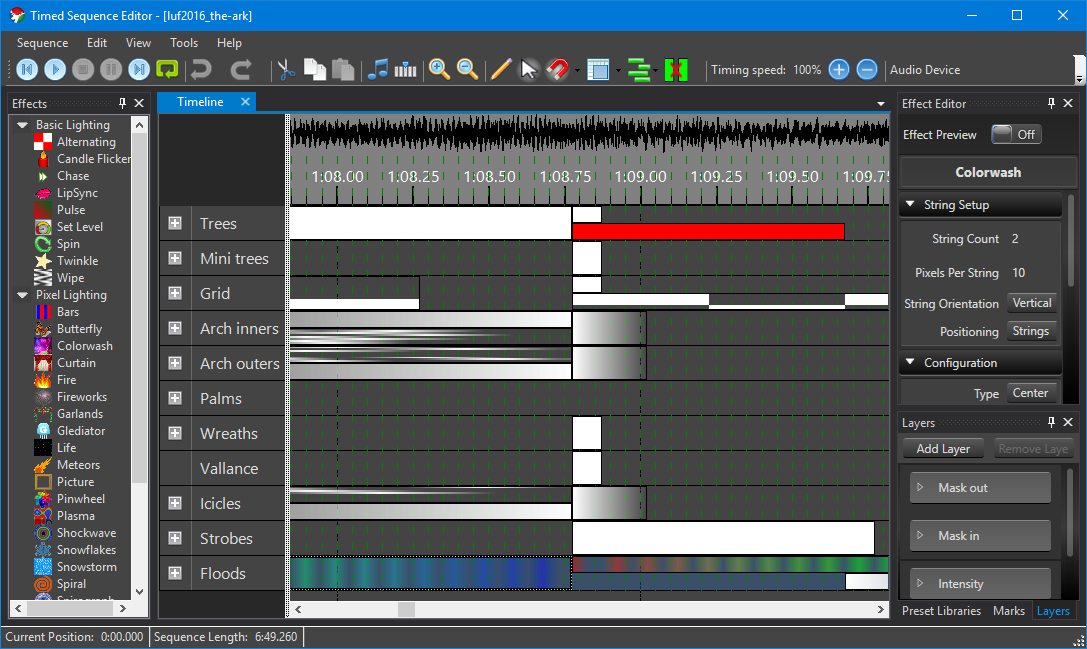
\includegraphics[width=0.9\textwidth]{Figs//vixen_editor.png}
  \caption{\footnotesize Vixen sequence editor interface}
  \label{fig:vixen-editor}
\end{figure}

Between elements and hardware controllers, filters are used to map the channel connections, and patches are used to define data linkages among them. Each element output may be discarded, duplicated or combined by the filters.

Inside each hardware controller module, data from multiple channels will be combined into a single data packet, then send through the appropriate hardware interface, which can be USB, Ethernet, etc. Each controller has its own update thread, with individual update frame rate settings.

Vixen has another dedicated configuration interface for controllers and filter connections, as shown by \fref{fig:vixen-setup}.

\begin{figure}[!t]
  \centering
  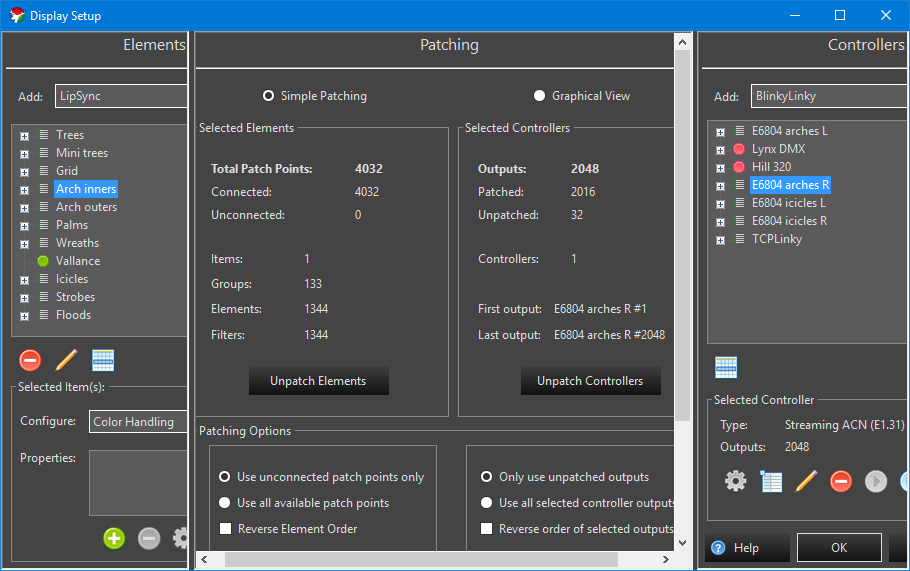
\includegraphics[width=0.9\textwidth]{Figs//vixen_setup.png}
  \caption{\footnotesize Vixen controller setup interface}
  \label{fig:vixen-setup}
\end{figure}

Vixen also has a preview display. It maps element outputs to sets of points on a 2D surface, possibly arranged as the shapes of actual physical objects. The preview was rendered on a separate window, as shown by \fref{fig:vixen-preview}.

\begin{figure}[!t]
  \centering
  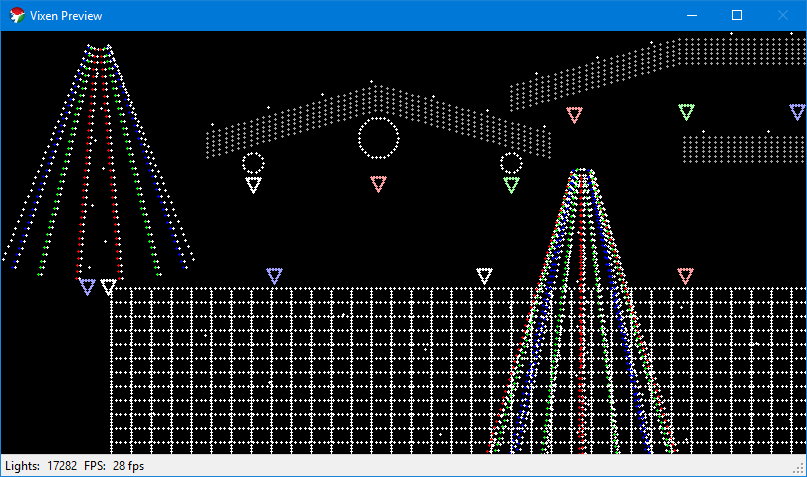
\includegraphics[width=0.9\textwidth]{Figs//vixen_preview.png}
  \caption{\footnotesize Vixen preview interface}
  \label{fig:vixen-preview}
\end{figure}

\section{Similar applications}

\cmt{Further background researches may need to be done, such as analysing other lighting control applications' performances and their implementations.}

\section{Testing platforms}

\subsection{Microsoft Windows based systems}

As the Vixen application was originally developed based on Microsoft Windows, so a mid-range laptop running Microsoft Windows 10 x64 was used as the primary development platform. It is capable of running Microsoft Visual Studio required for developing the Vixen application, but with relatively lower computation power to expose the run-time performance issue of Vixen.

This platform was also used to remotely connect to other development platforms, using technologies such as SSH.

The hardware specifications are listed below:

%\begin{enumerate}[noitemsep]
\begin{description}
  \item[CPU:]	Intel dual-core i5-3337U, 1.80 GHz
  \item[RAM:]	LPDDR3 8.0GB 1600MHz
  \item[Disk:]	Solid-state drive
\end{description}

\subsection{Linux based systems}
\label{sec:systems}

Multiple Linux based systems with a variety of resource configurations, ranging from high performance desktop platforms to low-end embedded platforms, were used for performance testing, as listed in \tref{tbl:linux}.

\begin{table}[!h]
  \centering
  \begin{tabular}{l|l|l|l|l}
    \hline
    \textbf{Name} & \textbf{Architecture} & \textbf{CPU} & \textbf{Specification} & \textbf{RAM} \\
    \hline
    NAS         & x86\_64 & AMD FX-8350       & 8 cores @ 4.0GHz  & 16GiB   \\ \hline
    Jetson TX2  & aarch64 & NVIDIA Tegra X2   & 6 cores @ 2.0GHz  & 8GiB    \\ \hline
    RPi 3B      & armv7l  & Broadcom BCM2837  & 4 cores @ 1.2GHz  & 1GiB    \\ \hline
    RPi Zero W  & armv6l  & Broadcom          & 1 core @ 1.0GHz   & 512MiB  \\ \hline
    RPi B+      & armv6l  & Broadcom BCM2835  & 1 core @ 900MHz   & 512MiB  \\ \hline
    Noah NP1380 & mipsel  & Ingenic JZ4740    & 1 core @ 336MHz   & 64MiB   \\ \hline
  \end{tabular}
  \caption{Linux based systems}
  \label{tbl:linux}
\end{table}

It is possible to install Microsoft Windows IoT system on some of the testing platforms. However, system, driver and runtime support were still not available for all of the testing platforms. Therefore, Debian \cite{debian} based Linux distributions including Ubuntu \cite{ubuntu} and Raspbian \cite{raspbian} were used on these systems.

\section{Microsoft .NET runtime}

\subsection{Microsoft Windows based}

Vixen runs on top of Microsoft's .NET runtime library \cite{platt2002introducing}, using C\# \cite{hejlsberg2003c} as the primary programming language, with the exception of a few dependency libraries written in C/C++.

The GUI of Vixen also relies on some legacy fragments of Windows Presentation Foundation (WPF) \cite{wpf}. Fortunately, the core functionality of Vixen does not require WPF, which makes it possible to be ported to Linux based systems.

\subsection{Linux based}

There were 3 possible ways to run Vixen on Linux based systems:

\begin{enumerate}
  \item Virtual machine emulation such as qemu \cite{qemu}
  \item Windows runtime emulation such as wine \cite{wine}
  \item Alternative .NET runtime implementation such as mono project \cite{de2004mono}
\end{enumerate}

Virtual machine emulation using qemu was possible on all testing platforms. However, emulation of x86 architecture on non-native ARM platforms requires instruction level emulation, which will be not be feasible with the computation power of the available systems. In addition, the entire Microsoft Windows operating system will also need to be emulated, further increasing the overhead even on native x86 platforms.

The overhead of running another operating system can be eliminated by using runtime emulators such as wine. However, runtime emulators require x86 platforms for running the x86 based Vixen application, not possible on ARM based embedded platforms.

The only possible solution was to using the mono project runtime implementation. Mono project is an up-to-date open source implementation of Microsoft .NET framework using C\#. It can translate executables developed using .NET framework directly to the host platform architecture during runtime, with techniques including Just-in-time (JIT) compiler. The functionalities of the executable will be JIT compiled as native code for the host. With the help of other native libraries, the overhead of using mono will be insignificant. Further more, mono project is available to a variety of processor architectures, including ARM and MIPS embedded platforms. Having Vixen running on an embedded platform can give greater flexibility.

\section{Codec libraries}

Since the overall process of Vixen lighting show is similar to video rendering, to support video format input, a multimedia codec library need to be used for decoding media files. It is impractical to implement numerous video decoding algorithms for different video formats in the time frame of this project, using an existing library would hide all the complicated implementation details.

For cross-platform support, an open source implementation would be more suitable. The most popular libraries are ffmpeg \cite{ffmpeg} and mencoder in mplayer \cite{mplayer}. The ffmpeg framework was chosen over mplayer, because it was more actively maintained with varies hardware acceleration capabilities.

Because the library binaries was used directly without modification to the source code, this should not violates the LGPL license ffmpeg was licensed by.

The ffmpeg framework consists of several individual libraries that would be useful to this project, as listed in \tref{tbl:ffmpeg}.

\begin{table}[!h]
  \centering
  \begin{tabular}{l|l}
    \hline
    \textbf{Name} & \textbf{Description} \\
    \hline
    libavcodec & Encoding/decoding library  \\ \hline
    libavfilter & Graph-based frame editing library \\ \hline
    libavformat & I/O and muxing/demuxing library   \\ \hline
    libavdevice & Special devices muxing/demuxing library \\ \hline
    libavutil & Common utility library    \\ \hline
    libswresample & Audio resampling, format conversion and mixing  \\ \hline
    libpostproc & Post processing library \\ \hline
    libswscale & Colour conversion and scaling library  \\ \hline
  \end{tabular}
  \caption{Different libraries provided by ffmpeg framework (sourced from \cite{ffmpeg})}
  \label{tbl:ffmpeg}
\end{table}

\section{Popular video encoding formats}

There are multiple format types for a single video file. First of all, a video container format will be needed to encapsulate different streams of data, such as video stream, audio stream and subtitle text stream. These formats specify how data elements are stored inside a single file, but does not specify the encoding or compression format used by individual data streams. Some examples of this type of formats includes mp4, avi and mkv.

For the video data stream, another set of encoding formats is used. For example, h265, h264, and mpeg. In addition, which colour space and colour channels will be used can also be specified. This is known as pixel format. It is often specified by combining colour channels, channel sizes and channel ordering together. The 2 most common colour spaces are YUV (luminance and chrominance) and RGB (red, green and blue). For example, pixel format "yuv444p" specifies colour space YUV with Y and UV channels taking 12 bytes per 4 pixels, and the channels are stored separately as planes. Similarly, pixel format "yuv420p" specifies YUV colour space with channels taking 6 bytes per 4 pixels, whereas "rgb24" specifies RGB colour space with R, G and B channels stored sequentially taking 3 bytes pre pixel.

\section{Audio rendering engine}

Unlike Microsoft Windows with definitive audio API, Linux has multiple audio libraries such as PulseAudio \cite{developers2013pulseaudio} and ALSA \cite{alsa} with complex audio framework structure. To simplify the underlying structure and enable cross-platform capability, the FMOD \cite{fmod} low-level API library was used. Despite being proprietary, it is available across Windows, Linux and also ARM based embedded platforms with unified easy-to-use API.

The original Vixen application already uses FMOD as a plugin in the original execution engine. However, the version it uses was out-dated without available documentation, and the plugin is only capable of playing audio files. Therefore, a more recent version was required. Furthermore, although the library has provided a set of C\# APIs, but the essential functionality required for playing custom audio stream was lacking, C/C++ APIs need to be used.

\section{Performance analysers}

Several performance analysers on different platforms was used through the project for optimisation and debugging purpose.

On Microsoft Windows, the built-in sampling profiler for Visual Studio was used. It samples the program stack frame multiple times during runtime without significant impact to program performance, analyses execution frequencies and duration of individual functions.

On Linux, the mono project also has profilers with sampling mode for analyse code segments that were written with C\# using .NET runtime. Linux also has sampling profilers for native programs, especially the perf profiler \cite{de2010new}. However, they can not provide much information about code written with intermediate languages such as C\# with .NET runtime.

\section{Performance profiling method}

In addition to profilers provided by the platform, performance profiling was also implemented within the Vixen application itself. It has relatively less overheads from generic profiling tools. However, it can only provide information specifically related to the execution engine, such as controller update frame rates. Therefore, the profiler was used only for overall execution performance comparison of the Vixen application.

The original profiler with Vixen uses the \texttt{Process} class provided by Microsoft Windows runtime for CPU usage measurements. However, it was not completely available under mono runtime. A different profiling method would be required for Linux.

On Linux, there are statistic files in the proc file system \cite{proc} provided by the kernel. Per-process information about CPU jiffies, disk I/O statistics are available by reading corresponding files.
